% Created by tikzDevice version 0.12.6 on 2025-05-16 11:07:58
% !TEX encoding = UTF-8 Unicode
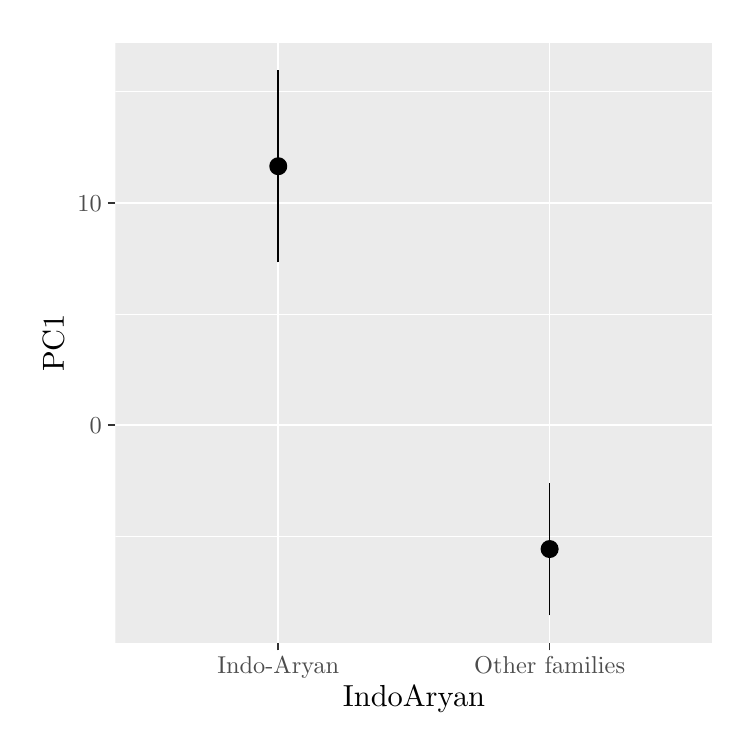
\begin{tikzpicture}[x=1pt,y=1pt]
\definecolor{fillColor}{RGB}{255,255,255}
\path[use as bounding box,fill=fillColor,fill opacity=0.00] (0,0) rectangle (252.94,252.94);
\begin{scope}
\path[clip] (  0.00,  0.00) rectangle (252.94,252.94);
\definecolor{drawColor}{RGB}{255,255,255}
\definecolor{fillColor}{RGB}{255,255,255}

\path[draw=drawColor,line width= 0.6pt,line join=round,line cap=round,fill=fillColor] (  0.00,  0.00) rectangle (252.94,252.94);
\end{scope}
\begin{scope}
\path[clip] ( 31.71, 30.69) rectangle (247.44,247.45);
\definecolor{fillColor}{gray}{0.92}

\path[fill=fillColor] ( 31.71, 30.69) rectangle (247.44,247.45);
\definecolor{drawColor}{RGB}{255,255,255}

\path[draw=drawColor,line width= 0.3pt,line join=round] ( 31.71, 69.06) --
	(247.44, 69.06);

\path[draw=drawColor,line width= 0.3pt,line join=round] ( 31.71,149.46) --
	(247.44,149.46);

\path[draw=drawColor,line width= 0.3pt,line join=round] ( 31.71,229.86) --
	(247.44,229.86);

\path[draw=drawColor,line width= 0.6pt,line join=round] ( 31.71,109.26) --
	(247.44,109.26);

\path[draw=drawColor,line width= 0.6pt,line join=round] ( 31.71,189.66) --
	(247.44,189.66);

\path[draw=drawColor,line width= 0.6pt,line join=round] ( 90.55, 30.69) --
	( 90.55,247.45);

\path[draw=drawColor,line width= 0.6pt,line join=round] (188.61, 30.69) --
	(188.61,247.45);
\definecolor{drawColor}{RGB}{0,0,0}

\path[draw=drawColor,line width= 0.6pt,line join=round] (188.61, 40.54) -- (188.61, 88.54);

\path[draw=drawColor,line width= 0.6pt,line join=round] ( 90.55,168.14) -- ( 90.55,237.59);
\definecolor{fillColor}{RGB}{0,0,0}

\path[draw=drawColor,line width= 0.8pt,line join=round,line cap=round,fill=fillColor] (188.61, 64.54) circle (  2.85);

\path[draw=drawColor,line width= 0.8pt,line join=round,line cap=round,fill=fillColor] ( 90.55,202.87) circle (  2.85);
\end{scope}
\begin{scope}
\path[clip] (  0.00,  0.00) rectangle (252.94,252.94);
\definecolor{drawColor}{gray}{0.30}

\node[text=drawColor,anchor=base east,inner sep=0pt, outer sep=0pt, scale=  0.88] at ( 26.76,106.23) {0};

\node[text=drawColor,anchor=base east,inner sep=0pt, outer sep=0pt, scale=  0.88] at ( 26.76,186.63) {10};
\end{scope}
\begin{scope}
\path[clip] (  0.00,  0.00) rectangle (252.94,252.94);
\definecolor{drawColor}{gray}{0.20}

\path[draw=drawColor,line width= 0.6pt,line join=round] ( 28.96,109.26) --
	( 31.71,109.26);

\path[draw=drawColor,line width= 0.6pt,line join=round] ( 28.96,189.66) --
	( 31.71,189.66);
\end{scope}
\begin{scope}
\path[clip] (  0.00,  0.00) rectangle (252.94,252.94);
\definecolor{drawColor}{gray}{0.20}

\path[draw=drawColor,line width= 0.6pt,line join=round] ( 90.55, 27.94) --
	( 90.55, 30.69);

\path[draw=drawColor,line width= 0.6pt,line join=round] (188.61, 27.94) --
	(188.61, 30.69);
\end{scope}
\begin{scope}
\path[clip] (  0.00,  0.00) rectangle (252.94,252.94);
\definecolor{drawColor}{gray}{0.30}

\node[text=drawColor,anchor=base,inner sep=0pt, outer sep=0pt, scale=  0.88] at ( 90.55, 19.68) {Indo-Aryan};

\node[text=drawColor,anchor=base,inner sep=0pt, outer sep=0pt, scale=  0.88] at (188.61, 19.68) {Other families};
\end{scope}
\begin{scope}
\path[clip] (  0.00,  0.00) rectangle (252.94,252.94);
\definecolor{drawColor}{RGB}{0,0,0}

\node[text=drawColor,anchor=base,inner sep=0pt, outer sep=0pt, scale=  1.10] at (139.58,  7.64) {IndoAryan};
\end{scope}
\begin{scope}
\path[clip] (  0.00,  0.00) rectangle (252.94,252.94);
\definecolor{drawColor}{RGB}{0,0,0}

\node[text=drawColor,rotate= 90.00,anchor=base,inner sep=0pt, outer sep=0pt, scale=  1.10] at ( 13.08,139.07) {PC1};
\end{scope}
\end{tikzpicture}
